% ─────────────────────────────────────────────────────────────────────────────
% local_mapper.tex
%
% Documentación incremental del módulo local_mapper.
% Cada versión agrega una sección que explica el componente incorporado.
% ─────────────────────────────────────────────────────────────────────────────

\section{Proyección de profundidad a coordenadas 3D}
\label{sec:lm-depth-projector}

El primer paso del pipeline de mapeo local consiste en transformar la imagen
de profundidad entregada por la cámara en una nube de puntos tridimensional
expresada en el sistema de coordenadas del sensor.

\subsection{Motivación}

La cámara de profundidad entrega, para cada píxel $(u, v)$, un valor entero
de 16 bits que representa la distancia al objeto en milímetros. Esta
representación es compacta y eficiente para transmisión, pero no es
directamente útil para razonamiento espacial: no permite saber si un
obstáculo se encuentra a la izquierda o a la derecha, ni a qué altura
respecto del suelo.

Para poder responder esas preguntas se necesita convertir cada píxel a un
punto $(x, y, z)$ en metros, en un sistema de coordenadas conocido. Esta
conversión se denomina \emph{retroproyección} y constituye la entrada
obligatoria de cualquier etapa posterior del pipeline (filtrado por altura,
alineación a gravedad, proyección a grilla de ocupación).

\subsection{Modelo pinhole}

La retroproyección utiliza el modelo de cámara pinhole. Los parámetros
intrínsecos de la cámara se obtienen del mensaje \texttt{CameraInfo}
publicado por el driver ROS del sensor. Los parámetros relevantes son:

\begin{itemize}
  \item $f_x$, $f_y$: distancias focales en píxeles (horizontal y vertical).
  \item $c_x$, $c_y$: coordenadas del punto principal (centro óptico) en
        píxeles.
\end{itemize}

Estos cuatro valores forman parte de la matriz de calibración intrínseca
$\mathbf{K}$ (de dimensión $3 \times 3$), de la cual se extraen las
posiciones $K_{0,0} = f_x$, $K_{1,1} = f_y$, $K_{0,2} = c_x$ y
$K_{1,2} = c_y$.

\subsection{Fórmulas de retroproyección}

Dado un píxel en la posición $(u, v)$ con valor de profundidad
$d_{\text{mm}}$ (en milímetros), la conversión a coordenadas 3D en metros
se realiza mediante:

\begin{align}
  z &= d_{\text{mm}} \times s \label{eq:depth-z} \\
  x &= \frac{(u - c_x) \cdot z}{f_x} \label{eq:depth-x} \\
  y &= \frac{(v - c_y) \cdot z}{f_y} \label{eq:depth-y}
\end{align}

\noindent donde $s = 10^{-3}$ es el factor de escala que convierte
milímetros a metros. El sistema de coordenadas resultante corresponde al
frame óptico de la cámara de profundidad
(\texttt{camera\_depth\_optical\_frame}):

\begin{itemize}
  \item $x$: eje horizontal, positivo hacia la derecha.
  \item $y$: eje vertical, positivo hacia abajo.
  \item $z$: eje de profundidad, positivo hacia la escena (adelante).
\end{itemize}

\subsection{Tratamiento de píxeles inválidos}

No todos los píxeles de la imagen de profundidad contienen mediciones
válidas. El sensor puede reportar un valor de 0 cuando el algoritmo de
correlación estéreo no logra establecer correspondencia entre las dos
imágenes infrarrojas, o de 65535 en caso de saturación. Estos píxeles
se descartan y se marcan como $(0, 0, 0)$ en la nube de puntos resultante.

Adicionalmente, el nodo aplica un filtro de rango: solo se conservan los
puntos cuya profundidad $z$ se encuentra dentro del intervalo
$[z_{\min}, z_{\max}]$ configurable. Esto elimina mediciones ruidosas
muy cercanas al sensor y puntos lejanos con baja confiabilidad.

\subsection{Implementación}

La clase \texttt{DepthProjector} encapsula la lógica de retroproyección.
Se construye a partir de un mensaje \texttt{CameraInfo} del cual extrae
los cuatro intrínsecos. Expone dos métodos:

\begin{itemize}
  \item \texttt{projectPixel(u, v, depth\_mm)}: retroproyecta un solo
        píxel.
  \item \texttt{projectDepthImage(data, w, h)}: retroproyecta la imagen
        completa, retornando un vector de puntos 3D.
\end{itemize}

El nodo \texttt{depth\_projection\_node} utiliza esta clase para suscribirse
a la imagen de profundidad y al \texttt{CameraInfo}, y publica el resultado
como un mensaje \texttt{PointCloud2} en el tópico
\texttt{/local\_mapper/debug/depth\_cloud}. Esta nube de puntos se puede
visualizar directamente en RViz para verificar que la proyección es
geométricamente correcta.

\subsection{Observaciones en RViz}

Al visualizar la nube de puntos publicada se observa:

\begin{enumerate}
  \item La forma tridimensional de los objetos presentes frente a la cámara,
        reconstruida fielmente a partir de la imagen de profundidad.
  \item Los puntos se encuentran en el frame óptico de la cámara, por lo
        que los objetos que están a la derecha del campo visual aparecen
        con valores positivos de $x$, y los que están debajo del centro
        óptico con valores positivos de $y$.
  \item Zonas sin puntos correspondientes a píxeles inválidos del sensor
        (superficies muy reflectivas, bordes de objetos o distancias fuera
        de rango).
  \item Toda la nube se encuentra ``cruda'': no está alineada a la gravedad
        ni compensada por la inclinación de la cámara. Si la cámara apunta
        ligeramente hacia abajo, el suelo aparece como un plano inclinado
        en lugar de horizontal.
\end{enumerate}

La Figura~\ref{fig:rviz-depth-cloud} muestra una captura de la
visualización en RViz, donde se presenta la nube de puntos coloreada por
eje $z$ junto con la imagen de color correspondiente del sensor. Esta
vista permite contrastar la escena real con la reconstrucción
tridimensional obtenida por retroproyección.

{\large\textcolor{red}{TO DO : cambiar imagenes para que sean 3 del mismo tamaño y angulo de
imagen. Utilizar las imagenes de medición con respecto a los cilindros de diferentes diametros a
diferentes distancias.}}

\begin{figure}[ht]
  \centering
  \begin{subfigure}[b]{0.32\textwidth}
    \centering
    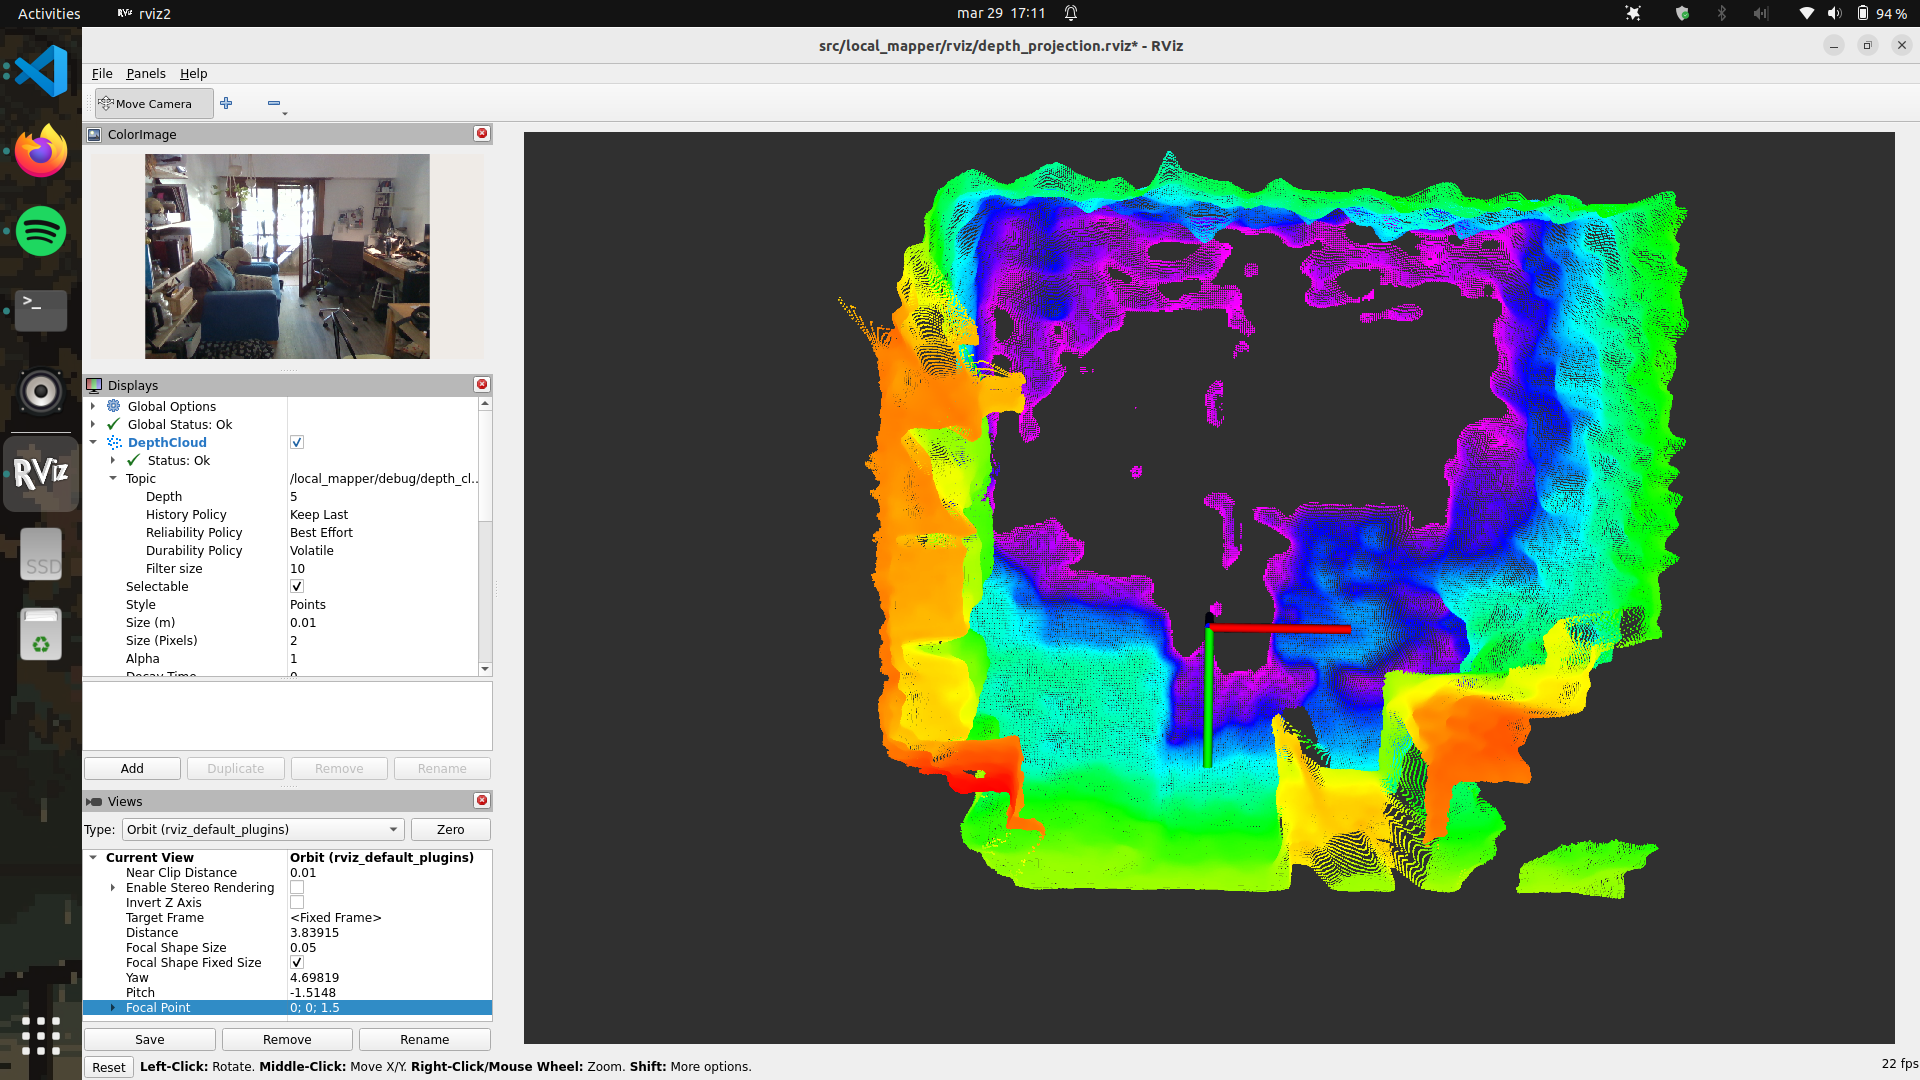
\includegraphics[width=\textwidth]{_Imagenes/mapeo/pinhole/rviz_depth_cloud.png}
    \caption{Habitación}
    \label{fig:depth-cloud-habitacion}
  \end{subfigure}
  \hfill
  \begin{subfigure}[b]{0.32\textwidth}
    \centering
    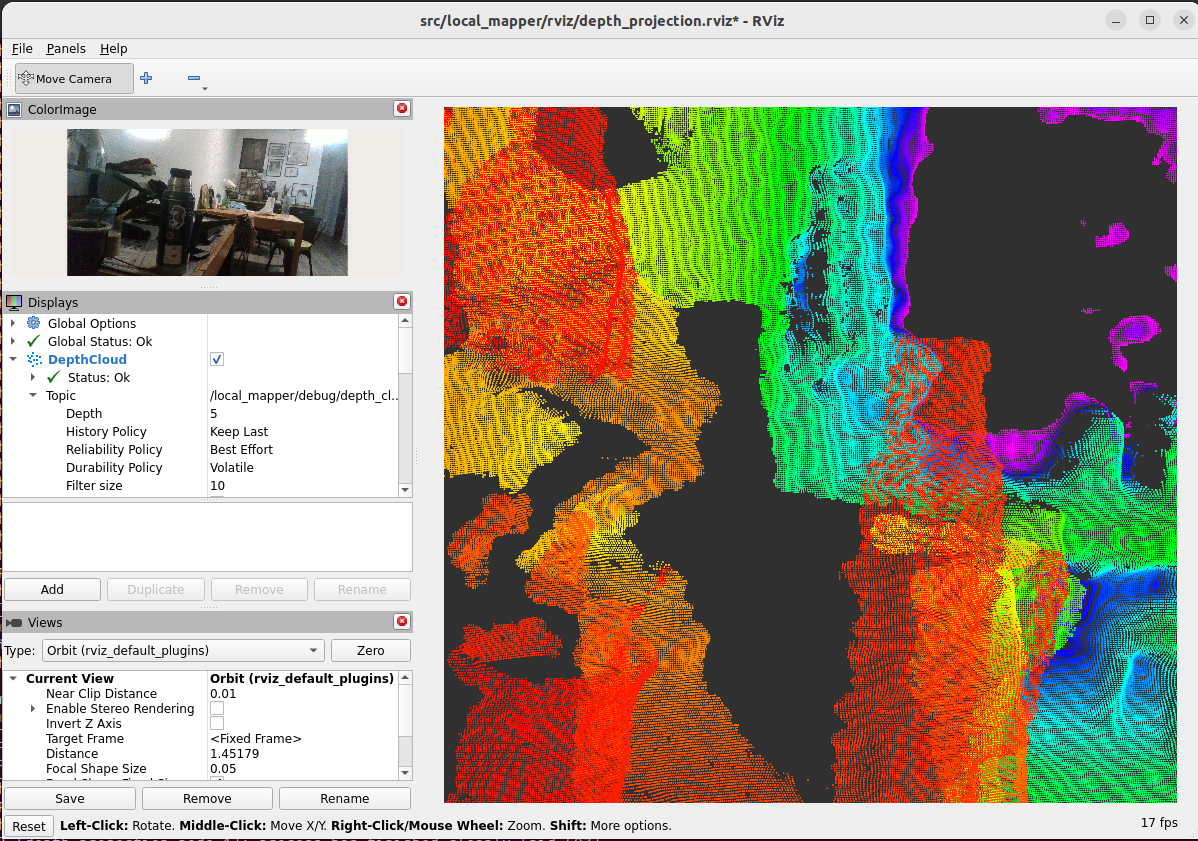
\includegraphics[width=\textwidth]{_Imagenes/mapeo/pinhole/ruido_objeto_cercano.png}
    \caption{Ruido en objeto cercano}
    \label{fig:depth-cloud-ruido-cercano}
  \end{subfigure}
  \hfill
  \begin{subfigure}[b]{0.32\textwidth}
    \centering
    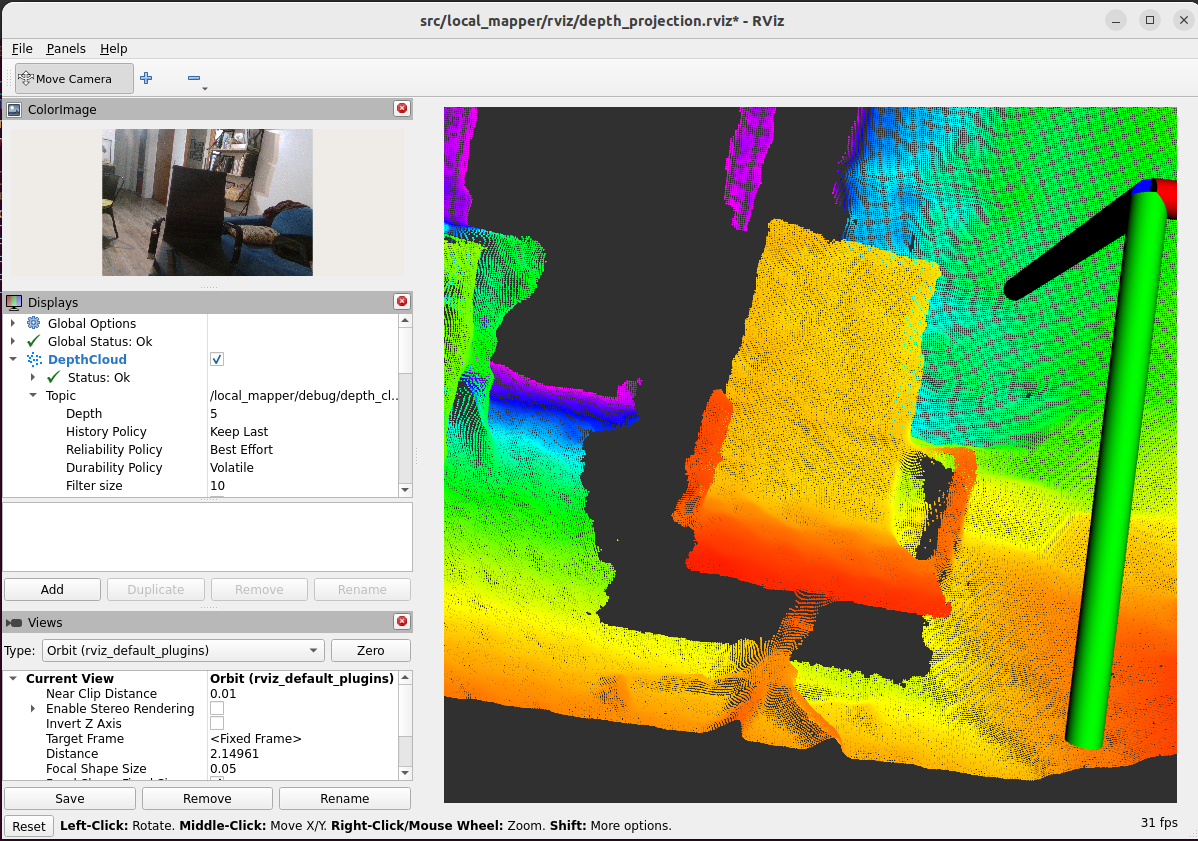
\includegraphics[width=\textwidth]{_Imagenes/mapeo/pinhole/ruido_objeto_1_5m.png}
    \caption{Ruido en objeto a 1{,}5\,m}
    \label{fig:depth-cloud-ruido-1-5m}
  \end{subfigure}
  \caption{Visualización en RViz de la nube de puntos retroproyectada
           y la imagen de color capturada por el sensor.
           La nube se colorea por profundidad en el eje $z$.}
  \label{fig:rviz-depth-cloud}
\end{figure}

Esta última observación motiva la necesidad del componente de alineación
gravitacional, que se aborda en la siguiente iteración del desarrollo.

\subsection{Ruido y limitaciones espaciales del sensor}

La visualización de la nube de puntos en RViz permite identificar con claridad
el comportamiento del ruido asociado al sensor de profundidad. A continuación
se describen las principales observaciones.

\subsubsection{Dependencia del ruido con la distancia}

El ruido en la nube de puntos aumenta progresivamente con la distancia al
sensor. A distancias cortas, la dispersión de los puntos es reducida y los
objetos se reconstruyen con alta fidelidad geométrica. A medida que la
distancia aumenta, la incertidumbre en la medición de profundidad se amplifica,
produciendo nubes más dispersas y superficies que visualmente aparecen
``rugosas'' o fragmentadas.

Este comportamiento es inherente al principio de operación de la cámara
estéreo: la precisión de la correspondencia entre las dos imágenes infrarrojas
disminuye cuando la disparidad entre ellas es pequeña, condición que se da
precisamente cuando los objetos están lejos del sensor.

\subsubsection{Filtrado de objetos pequeños a distancia}

Una consecuencia directa del aumento del ruido con la distancia es la pérdida
de capacidad para detectar objetos de pequeño tamaño. A corta distancia, el
sensor logra capturar con suficiente resolución objetos delgados o de sección
reducida. Sin embargo, al alejarse, estos objetos pueden quedar enmascarados
por el ruido o simplemente no generar suficientes píxeles válidos como para
ser reconocibles en la nube de puntos.

Este fenómeno representa una limitación crítica para el sistema en su conjunto,
dado que uno de sus objetivos es alertar al usuario sobre obstáculos que
normalmente pasan desapercibidos. El caso más representativo es el de cables
suspendidos a la altura de la cabeza: estructuras de sección milimétrica que,
dependiendo de la distancia a la que se encuentren, podrían no ser capturadas
por el sensor y, por ende, no ser transmitidas hapticamente al usuario.

\subsubsection{La resolución espacial como diferencial del sistema}

La resolución espacial es precisamente uno de los aspectos que distinguen al
uso de una cámara estéreo de profundidad frente a otras alternativas de
percepción del entorno, como sensores LiDAR de baja densidad o sensores
ultrasónicos. La densidad de la nube de puntos generada permite, en principio,
representar objetos con un nivel de detalle geométrico alto. Sin embargo, esta
ventaja solo se mantiene dentro de un rango de distancias donde el ruido no
degrada la medición por debajo de un umbral de utilidad práctica.

\subsubsection{Caracterización formal de la capacidad de detección}

Con el objetivo de cuantificar esta limitación y establecer criterios de
diseño para el sistema háptico, se llevó a cabo una caracterización formal
de la capacidad de detección del sensor en función de la distancia y del
tamaño del objeto. El procedimiento consistió en posicionar objetos cilíndricos
de diámetros conocidos (representativos de cables y barras) a distintas
distancias frente al sensor, bajo condiciones de iluminación controlada y
fondo homogéneo.

Para cada combinación de distancia y diámetro se adquirieron múltiples
capturas de la nube de puntos y se evaluó si el objeto era detectable como
una estructura coherente, definiendo detección como la presencia de al menos
un conjunto mínimo de puntos válidos con la geometría esperada. Se tabularon
así los pares (distancia, diámetro) que se encontraban en la frontera de
detección, obteniendo una curva límite que caracteriza el sensor.

Esta curva permite responder preguntas concretas del diseño: dado un objeto
de cierta sección transversal, a qué distancia máxima puede ser detectado de
forma confiable, y cuál es la distancia mínima a la que el sistema háptico
debe advertir al usuario para que la información sea accionable.

{\large\textcolor{red}{TO DO : Realizar medición/experimento}}

\begin{table}[h]
\centering
\caption{Caracterización del sensor Intel RealSense D435i}
\label{tab:d435i_caracterizacion}
\begin{tabular}{ccccc}
\toprule
\textbf{Distancia} & \textbf{$\bar{Z}$ (m)} & \textbf{$\sigma_Z$ (mm)} & \textbf{Flying pixels (\%)} & \textbf{FPS estable} \\
\midrule
0{,}5 m & -- & -- & -- & -- \\
1{,}0 m & -- & -- & -- & -- \\
2{,}0 m & -- & -- & -- & -- \\
3{,}0 m & -- & -- & -- & -- \\
\bottomrule
\end{tabular}
\begin{tablenotes}
  \small
  \item $\bar{Z}$: media de profundidad sobre ROI central de $100 \times 100$ px.
  \item $\sigma_Z$: desviación estándar de $Z$ (ruido axial RMS).
  \item Flying pixels: porcentaje de píxeles con \texttt{depth = 0} o \texttt{depth = 65535}.
  \item FPS medido sobre 300 frames con \texttt{ros2 topic hz}.
  \item Superficie de referencia: pared plana, iluminación interior estándar.
\end{tablenotes}
\end{table}
